\documentclass[tikz,border=6pt]{standalone}
\usepackage{amsmath,amssymb,mathtools,physics,bm,nicefrac,wasysym}
\usepackage{xcolor}

\definecolor{colone}{RGB}{180,60,60}
\definecolor{coltwo}{RGB}{60,110,180}
\definecolor{colthree}{RGB}{60,140,80}

\definecolor{accent}{HTML}{A13D2C}
\definecolor{accent2}{HTML}{2B5F6B}
\definecolor{muted}{HTML}{5A564F}
\definecolor{panel}{HTML}{F8F6F0}
\definecolor{linecol}{HTML}{D8D2C4}
\definecolor{ink}{HTML}{1E1C1A}
\definecolor{astroblue}{HTML}{1B4F72}
\definecolor{astrodark}{HTML}{17202A}
\definecolor{sunyellow}{HTML}{E8A33D}

\usetikzlibrary{calc,arrows.meta,positioning,decorations.pathreplacing,decorations.markings,angles,quotes,shapes.geometric}
\usepackage{tikz-3dplot}

\newcommand{\vecr}{\vec r}
\newcommand{\vecL}{\vec L}
\newcommand{\vecA}{\vec A}
\newcommand{\vecf}{\vec f}
\newcommand{\vecF}{\vec F}
\newcommand{\vecp}{\vec p}
\newcommand{\avg}[1]{\left\langle #1\right\rangle}
\newcommand{\vecx}{\vec x}
\newcommand{\hatn}{\hat n}
\newcommand{\rhat}{\hat r}
\newcommand{\phihat}{\hat\phi}
\newcommand{\thetahat}{\hat\theta}
\newcommand{\note}[1]{\textcolor{blue!60!black}{\textit{[#1]}}}

\newcommand{\LST}{\mathrm{LST}}
\newcommand{\GST}{\mathrm{GST}}
\newcommand{\GMST}{\mathrm{GMST}}
\newcommand{\GAST}{\mathrm{GAST}}
\newcommand{\LMST}{\mathrm{LMST}}
\newcommand{\LAST}{\mathrm{LAST}}
\newcommand{\UT}{\mathrm{UT}}
\newcommand{\UTC}{\mathrm{UTC}}
\newcommand{\TAI}{\mathrm{TAI}}
\newcommand{\TT}{\mathrm{TT}}
\newcommand{\TDB}{\mathrm{TDB}}
\newcommand{\JD}{\mathrm{JD}}
\newcommand{\MJD}{\mathrm{MJD}}
\newcommand{\EoT}{\mathrm{EoT}}
\newcommand{\SNR}{\mathrm{SNR}}
\newcommand{\RON}{\mathrm{RON}}



\begin{document}
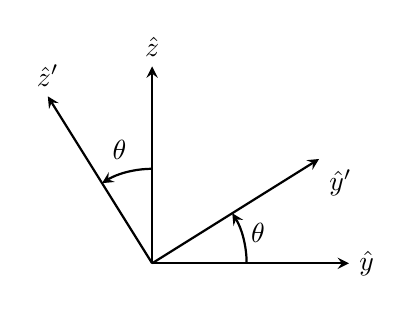
\begin{tikzpicture}[>=stealth, line width=0.8pt]
    			% Origin
    			\coordinate (O) at (0,0);
    			
    			% Parameters
    			\def\thetaVal{-32} % Rotation angle in degrees
    			\def\len{2.5}     % Length of axis vectors
    			
    			% Original coordinate axes
    			\draw[->] (O) -- (\len, 0) node[right] {$\hat{y}$};
    			\draw[->] (O) -- (0, \len) node[above] {$\hat{z}$};
    			
    			% Rotated coordinate axes (clockwise by \thetaVal)
    			\draw[->] (O) -- (-\thetaVal:\len) node[below right] {$\hat{y}'$};
    			\draw[->] (O) -- (90-\thetaVal:\len) node[above] {$\hat{z}'$};
    			
    			% Angle arc between y and y'
    			\draw[->] (0, 1.2) arc (90:90-\thetaVal:1.2);
    			\node at (90-\thetaVal/2: 1.5) {$\theta$};
    			
    			% Angle arc between x and x'
    			\draw[->] (1.2, 0) arc (0:-\thetaVal:1.2);
    			\node at (-\thetaVal/2: 1.4) {$\theta$};
    		\end{tikzpicture}
\end{document}
